\documentclass[12pt]{article}
\usepackage[a4paper, margin=2cm]{geometry}
\usepackage[english]{babel} % To obtain English text with the blindtext package
\usepackage{blindtext}
\usepackage{graphicx} % Required for inserting images
\usepackage{array, multirow} % For extra column formatting
\usepackage{amsmath, amssymb, cancel} %for equation environment
\usepackage{float}
\usepackage{parskip} % For gaps between para
\usepackage{setspace}
\usepackage{pdfpages}
\usepackage{abstract}
\usepackage[export]{adjustbox}
\usepackage{emptypage}
\usepackage{tocloft}
\usepackage[nottoc]{tocbibind}
\usepackage{hyperref, url}
\usepackage[table]{xcolor}
\usepackage{minted}
    \usemintedstyle{monokai}
\usepackage{caption,subcaption}
    \captionsetup{font=footnotesize,labelfont=bf}
\usepackage{tcolorbox}
    \newtcolorbox{mintedbox}{
        colback=backcolour,
        boxrule=0pt,
        sharp corners,
        width=\linewidth,
        left=0pt, right=0pt,
        top=3pt, bottom=3pt
    }

\cftsetindents{section}{0em}{2em}
\cftsetindents{subsection}{0em}{2em}

\renewcommand\cfttoctitlefont{\hfill\Large\bfseries}
\renewcommand\cftaftertoctitle{\hfill\mbox{}}

\graphicspath{ {./images/} }

\definecolor{blurple}{HTML}{5865F2}
\definecolor{backcolour}{HTML}{272823}

\hypersetup{
    colorlinks=true,
    linkcolor=black,
    urlcolor=black,
    citecolor=blurple,
}

\urlstyle{same}

\renewcommand{\arraystretch}{1.3}

\setcounter{secnumdepth}{5}
\setcounter{tocdepth}{5}
\newcommand\simpleparagraph[1]{%
  \stepcounter{paragraph}\paragraph*{\theparagraph\quad{}#1}}

\pagenumbering{arabic}

%%%%%%%%%%%%%%%%%%%%%%%%%%%%%%%%%%%


\title{PHYC20040 Exp.4 Asteroids}
\author{Joana Adao}
\date{\today}

\begin{document}

\begin{titlepage}
    \begin{center}

        \begin{figure}[ht]
            
\includegraphics[width=\textwidth]{UCDLogo.png}
        \end{figure}
        
        \begin{figure}
            \centerline{
\includegraphics[width=\paperwidth]{UCDBanner.png}}
        \end{figure}

        \vspace{4cm}

        {\LARGE \bfseries PHYC20040 Exploring the Solar System}\\
        \vspace{0.75cm}
        {\Large Experiment No.4 Astrometry of Asteroids}
        
        \vspace{1cm}
    
    {\Large \textbf{26 March 2025}}

    \vspace{2cm}
    
    {\large \textbf{by Joana C.C. Adao (Student No. 23311051)}}\\

    \end{center}

   \clearpage

\end{titlepage}

\tableofcontents
\thispagestyle{empty}

\newpage

\begin{abstract}
\addtocontents{toc}{\protect\contentsline{section}{\textbf{Abstract}}{\hfill}{}}
\thispagestyle{empty}



 
\end{abstract}
\newpage

%%%%%%%%%%%%%%%%%%%%%%%%%%%%%%%%%%%

\setcounter{page}{1}
\section{Theory} \label{sec:1}

\subsection{Introduction to Astrometry}

Astrometry is a type of astronomical measurement technique that focuses specifically on measuring the location of moving celestial objects within the sky plane \cite{ENDL2007887}.
This was one of the first techniques developed for searching planets around other stars, and remains a fundamental tool to astronomers to this day \cite{UCDastrometry,ENDL2007887}.

There are, of course, standard errors that come from measuring the movement of celestial objects through astrometric observations. This applies to both one's personal measurements and those found in star catalogues.
There will always be noise error when collecting photons from the targets, whether that be from background noise or from the target itself, photon distribution will vary between measurements at each different exposure time \cite{owen2000error}.
When measuring the position of an asteroid there will be tracking errors due to the fact that astroids move, sometimes producing trails that are neither straight nor uniformly illuminated, hence determining the centre is difficult \cite{owen2000error}.
These are examples of random errors that can be encountered, but there also exist systematic errors. The reference star catalogue may have possible zone errors, meaning stars have a bias for a particular region
of the sky that apply to any other asteroid measured in that sky region. The Hipparcos mission (1989-1993) was able to better pinpoint star's motion and position, thus effectively lessening this error \cite{owen2000error} and is being further
refined by the Gaia mission (2013-2025) \cite{hipparcos,gaiaesa}.

\subsection{Equatorial Coordinates}



\begin{figure}[H]
    \centering
    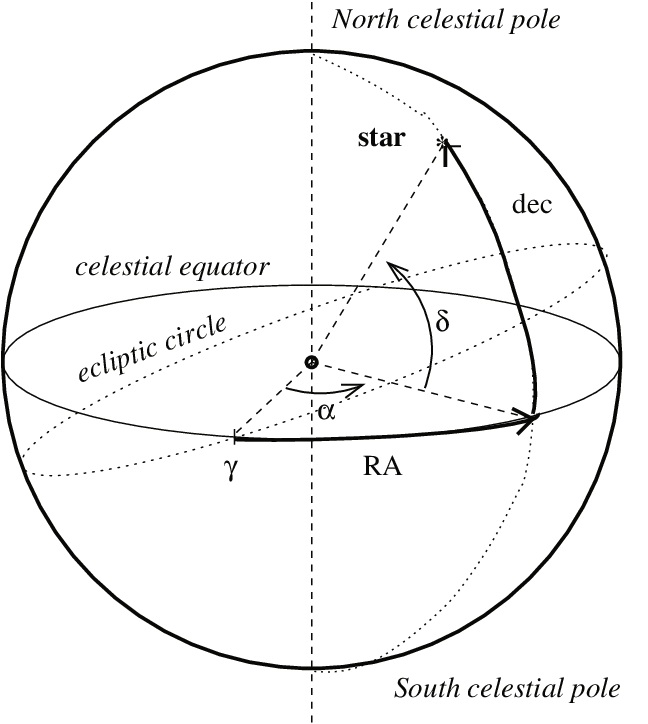
\includegraphics[width=.5\textwidth]{equatorial coords.png}
    \caption{Definition of equatorial coordinates system on the sky. Observer is at the centre of the sphere, which has an arbitrary radius of $\infty$ \protect\cite{equatorialcoords}.}
    \label{fig:1}
\end{figure}

\subsubsection{Right Ascension and Declination}



\subsubsection{Reference Star Catalogues}

\textbf{FK5} \cite{warren1990fifth}.

\textbf{Hubble Space Telescope Guide Star Catalogue (HST GSC)} \cite{hstgsc}.

\subsection{Celestial Coordinates}



\subsection{Principles of Parallax}






\section{Methodology} \label{sec:2}



\section{Results and Discussion} \label{sec:3}



\section{Conclusion} \label{sec:4}



\newpage

%%%%%%%%%%%%%%%%%%%%%%%%%%%%%%%%%%%

\bibliographystyle{IEEEtran}
\bibliography{References} \label{sec:ref}

\vspace{1.5cm}

\listoffigures


\end{document}